\documentclass[12pt]{article}

\newcommand{\name}{Mike Gao}
\newcommand{\problemset}{ MIDTERM }

%\pagestyle{headings}
\usepackage[dvips]{graphics,color}
\usepackage{amsfonts}
\usepackage{amssymb}
\usepackage{amsmath}
\usepackage{latexsym}
\usepackage{enumerate}
\usepackage{listings}
\usepackage{graphicx}
\setlength{\parskip}{1pc}
\setlength{\parindent}{0pt}
\setlength{\topmargin}{-3pc}
\setlength{\textheight}{9.5in}
\setlength{\oddsidemargin}{0pc}
\setlength{\evensidemargin}{0pc}
\setlength{\textwidth}{6.5in}

\newcommand{\answer}[1]{
\newpage
\noindent
\framebox{
	\vbox{
		COMP 557 \hfill {\bf \problemset} \hfill Prof. Paul Kry \\ 
		\name \hfill \today \\
		260915701 \hfill \# #1
	}
}
\bigskip

}
\usepackage{xcolor}

\definecolor{commentsColor}{rgb}{0.497495, 0.497587, 0.497464}
\definecolor{keywordsColor}{rgb}{0.000000, 0.000000, 0.635294}
\definecolor{stringColor}{rgb}{0.558215, 0.000000, 0.135316}

\lstset{ %
  backgroundcolor=\color{white},   % choose the background color; you must add \usepackage{color} or \usepackage{xcolor}
  basicstyle=\footnotesize,        % the size of the fonts that are used for the code
  breakatwhitespace=false,         % sets if automatic breaks should only happen at whitespace
  breaklines=true,                 % sets automatic line breaking
  captionpos=b,                    % sets the caption-position to bottom
  commentstyle=\color{commentsColor}\textit,    % comment style
  deletekeywords={...},            % if you want to delete keywords from the given language
  escapeinside={\%*}{*)},          % if you want to add LaTeX within your code
  extendedchars=true,              % lets you use non-ASCII characters; for 8-bits encodings only, does not work with UTF-8
  frame=tb,	                   	   % adds a frame around the code
  keepspaces=true,                 % keeps spaces in text, useful for keeping indentation of code (possibly needs columns=flexible)
  keywordstyle=\color{keywordsColor}\bfseries,       % keyword style
  language=c,                    % the language of the code (can be overrided per snippet)
  otherkeywords={*,...},           % if you want to add more keywords to the set
  numbers=left,                    % where to put the line-numbers; possible values are (none, left, right)
  numbersep=5pt,                   % how far the line-numbers are from the code
  numberstyle=\tiny\color{commentsColor}, % the style that is used for the line-numbers
  rulecolor=\color{black},         % if not set, the frame-color may be changed on line-breaks within not-black text (e.g. comments (green here))
  showspaces=false,                % show spaces everywhere adding particular underscores; it overrides 'showstringspaces'
  showstringspaces=false,          % underline spaces within strings only
  showtabs=false,                  % show tabs within strings adding particular underscores
  stepnumber=1,                    % the step between two line-numbers. If it's 1, each line will be numbered
  stringstyle=\color{stringColor}, % string literal style
  tabsize=2,	                   % sets default tabsize to 2 spaces
  title=\lstname,                  % show the filename of files included with \lstinputlisting; also try caption instead of title
  columns=fixed                    % Using fixed column width (for e.g. nice alignment)
}

\begin{document}


% PROBLEM 1

\answer{1 -- Coordinate Frame}

\begin{lstlisting}
// normal vector is n, n dot p is the point, let s, t be coordinates
Matrix4d coordFrame( const Vec3f &n, const Vec3f &p)
{
  // if it is near x axis
  Vec3f s,t;
  if(n.x > 0.9f) {
    s = Vec3f (0.0 f, 1.0 f, 0.0 f );
  } else {
    s = Vec3f (1.0 f, 0.0 f, 0.0 f);
  }
  s -= n* dot(s, n); // make s orthogonal to n
  s *= rsqrt(dot(s, s)); // normalize s
  t = cross(n, s);
  return (new double[] {
    t.x, s.x, n.x, p.x,
    t.y, s.y, n.y, p.y,
    t.z, s.z, n.z, p.z
    0, 0, 0, 1
  })
}
\end{lstlisting}


% PROBLEM 2

\answer{2 --  Rotation Using Similarity Transform}


Assume the axis pass through $(x_1, y_1, z_1)$ and $(x_2, y_2, z_2)$
\begin{enumerate}[(1)]

\item
Create the axis passing through origin by translating space by $-P_1$ for example

$ T = \begin{pmatrix}
1 & 0 & 0 & -x_1\\
0 & 1 & 0 & -y_1\\
0 & 0 & 1 & -z_1\\
0 & 0 & 0 & 1
\end{pmatrix}$

\item
Rotate axis into one of the original axis, Fix z, let u be a unit vector $(p,q,r)$

Project $u$ onto yz-plane to get $u'$ and rotate by $\alpha$ in order to get $u$ in xz-plane

$u'=\sqrt{q^2+r^2}$, $cos\alpha = r/u' $ $sin\alpha = q/u'$
$ Rx = \begin{pmatrix}
1 & 0 & 0 & -x_1\\
0 & \frac{r}{u'} & -\frac{q}{u'} & 0\\
0 & \frac{q}{u'} & \frac{r}{u'} & 0\\
0 & 0 & 0 & 1
\end{pmatrix}$

\item
We then rotate $u'$ to overlap z-axis, $cos\beta = u'/||u|| = u'$ $sin\beta = p/||u|| = p $
$ Ry = \begin{pmatrix}
u' & 0 & -p & 0\\
0 & 1 & 0 & 0\\
p & 0 & u & 0\\
0 & 0 & 0 & 1
\end{pmatrix}$

\item
We then rotate around z-axis by $\theta$
$ Rz = \begin{pmatrix}
cos\theta & -sin\theta & 0 & 0\\
sin\theta & cos\theta & 0 & 0\\
0 & 0 & 1 & 0\\
0 & 0 & 0 & 1
\end{pmatrix}$

Finally, $M=T^{-1}R_x^{-1}R_y^{-1}R_zR_yR_xT$
\end{enumerate}



% PROBLEM 3

\answer{3 -- Perspective Projection Matrix}

$ P = \begin{pmatrix}
n & 0 & 0 & 0\\
0 & n & 0 & 0\\
0 & 0 & n & 0\\
0 & 0 & -1 & 0
\end{pmatrix}$

Where this will take in point $(x, y, z, -1)^T$ to $(nx, ny, nz, -z)^T$, After dividing by the $z$ coordinate we have $(-nx/z,-ny/z,n,-1)$ which is the desired point of the near plane



% PROBLEM 4

\answer{4 -- Creating Similarity Transform to Provide Cheap Shadow Projection}



% PROBLEM 5

\answer{5 -- What is the closest near plane you can set?}

Let $s=\begin{pmatrix}0\\0\\-1\\1\end{pmatrix}$ be a point on the quadrilateral, and $t=\begin{pmatrix}0\\0\\-2\\1\end{pmatrix}$ be a point on the wall.

$P =\begin{pmatrix}n&0&0&0\\0&n&0&0\\0&0&n+10&10n\\0&0&-1&0\end{pmatrix}$

$P_s = \begin{pmatrix}0\\0\\-n-10+10n\\1\end{pmatrix}$

$P_t = \begin{pmatrix}0\\0\\-2n-20+10n\\2\end{pmatrix} =  \begin{pmatrix}0\\0\\-n-10+5n\\1\end{pmatrix}$

We are only concerned about the z coordinates of those points

$z_{P_s} = -n-10+10n$

$z_{P_t} = -n-10+5n$

We want to minimize, i.e $|z_{P_s} - z_{P_t}| = \epsilon$ so:

$|-n-10+10n-(-n-10+5n)| = \epsilon$

$|5n| = \epsilon$

$n=\frac{\epsilon}{5}$

% PROBLEM 6

\answer{6 -- Where Should the Point Light Be Placed?}
\begin{center}
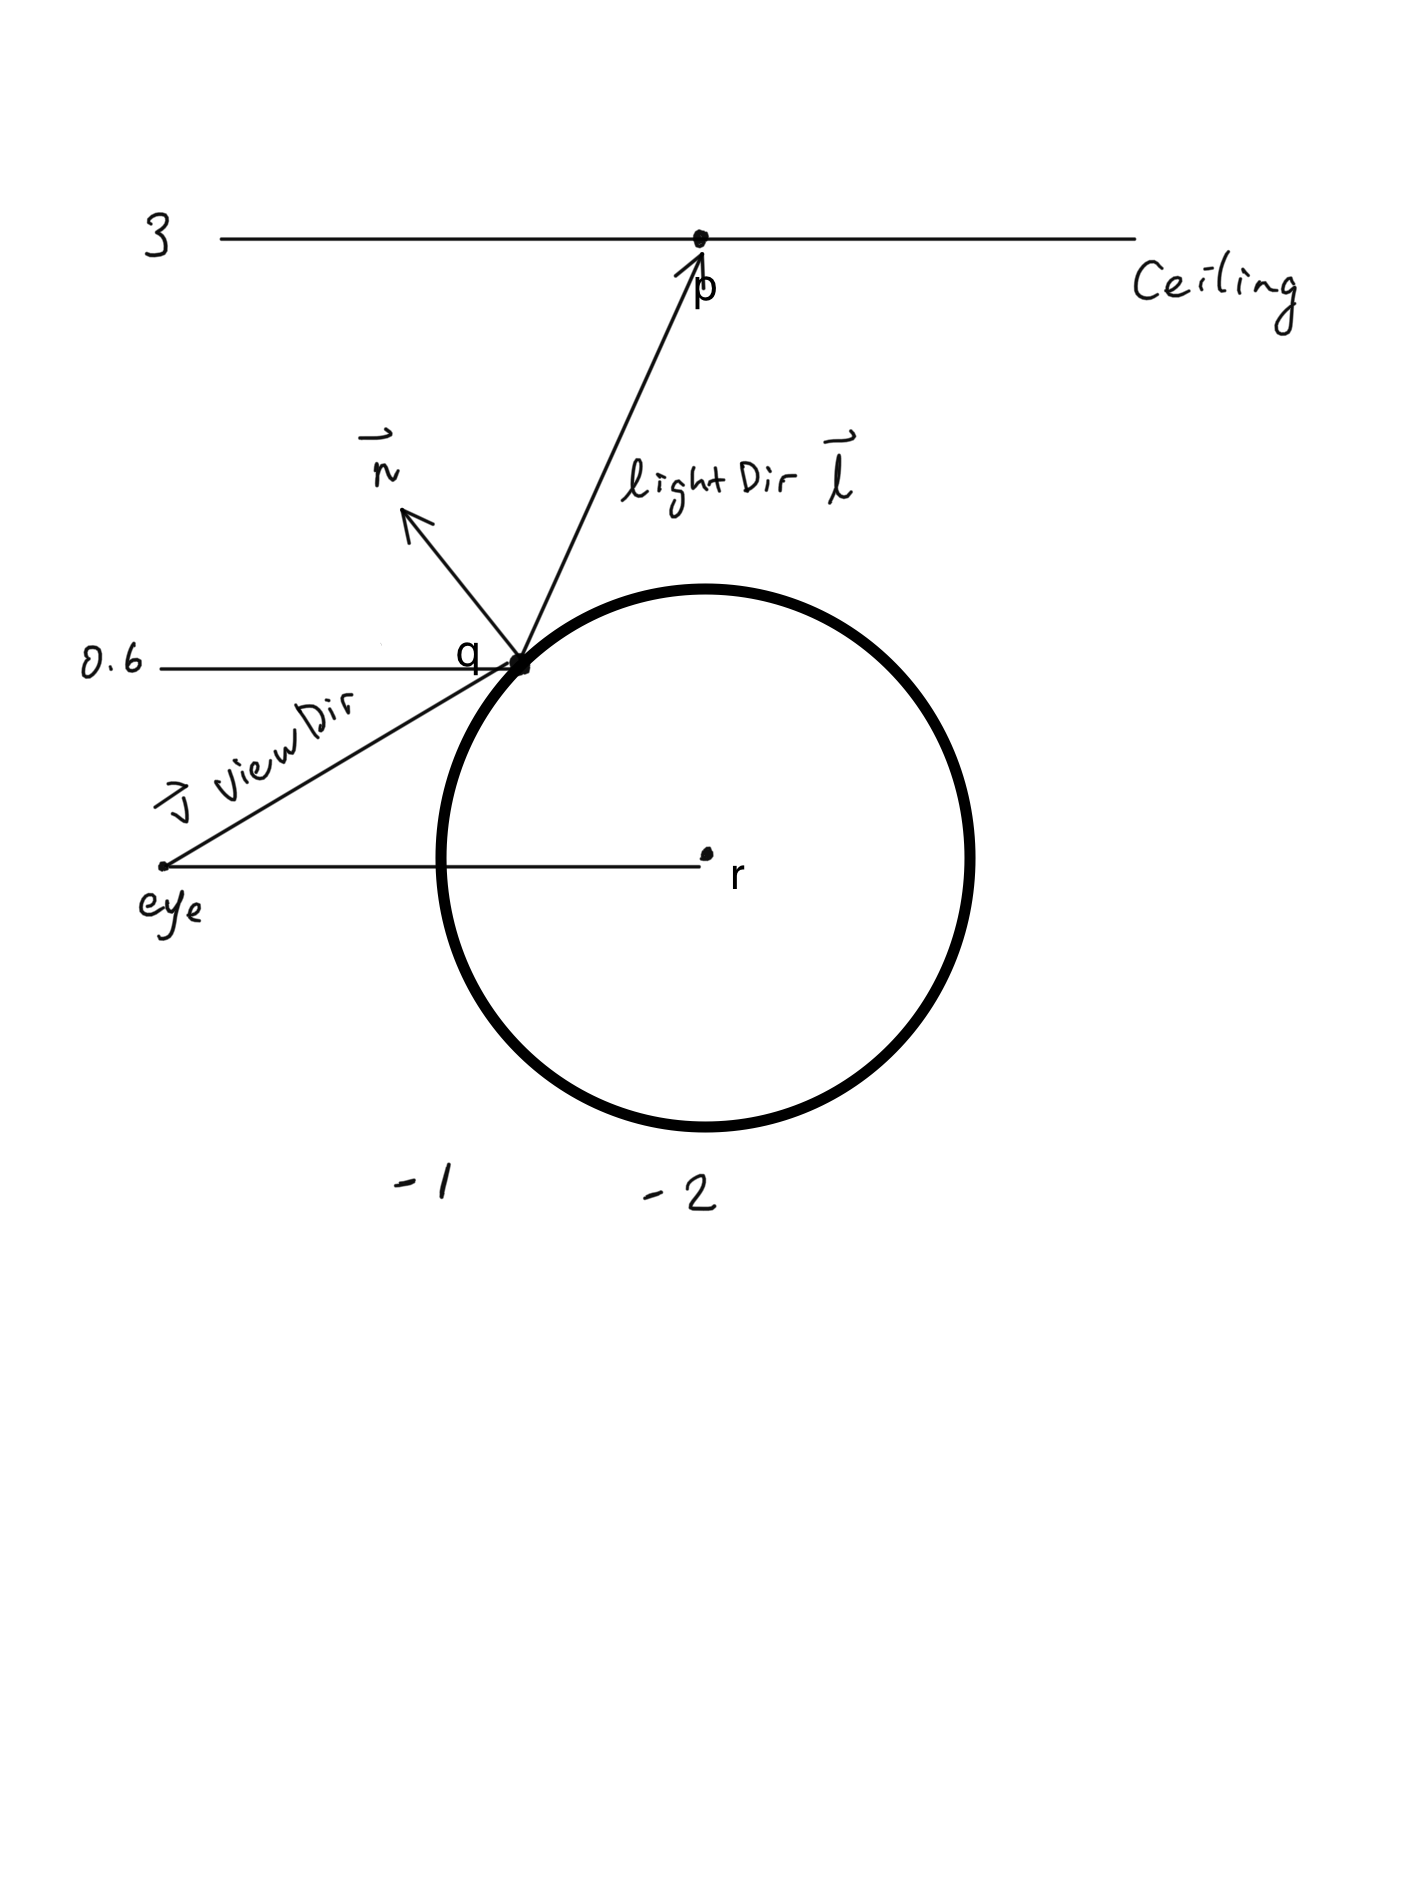
\includegraphics[width=14cm, height=19cm]{q6-diagram.png}
\end{center}
Where p is the light position (unknown), r is the center of the circle, q is the brightest spot of a
Blinn-Phong specular highlight.

We need to find the position of $q$ first. Since we know $y_q = 0.6$, we get:

$x_q^2+0.6^2=1$

$x_q =0.8$

Thus, $z_q = -2+0.8 = 1.2$

Now we can find the view direction $v$ and the normal $n$.

$n = q-r = \begin{pmatrix}0 \\0.6\\0.8\\0\end{pmatrix}$

$v = eye - q = \begin{pmatrix}0 \\-0.6\\1.2\\0\end{pmatrix}$

Now let's find $l$. Suppose $u$ is a vector such that $v - 2u = l$

$u = v - proj_n v = \begin{pmatrix}0 \\-0.6\\1.2\\0\end{pmatrix}- \begin{pmatrix}0\\0.36\\0.48\\0\end{pmatrix} =\begin{pmatrix}0\\-0.96\\0.72\\0\end{pmatrix}$


$l = v-2u=\begin{pmatrix}0 \\-0.6\\1.2\\0\end{pmatrix}-2\begin{pmatrix}0 \\-0.96\\0.72\\0\end{pmatrix}=\begin{pmatrix}0 \\1.32\\-0.24\\0\end{pmatrix}$

Now let's find out the location of the Light

Parametric equations of the direction: $x=0 \quad y=0.6+1.32t \quad z=-1.2-0.24t$

Equation of the ceiling:$y=3$

$3=0.6+1.32t$

$t=\frac{20}{11}$

$z=-1.2 - 0.24t$

$z=-\frac{18}{11}$

So the light should be at $\begin{pmatrix}0\\3\\-\frac{18}{11}\\1\end{pmatrix}$

% PROBLEM 7

\answer{7 -- Debug the Given Bling Phong Implementation}

Vertex Shader
\begin{lstlisting}
#version 400 core
uniform mat4 M;
// modeling matrix
uniform mat4 V;
// view matrix
uniform mat4 P;
// projection matrix
uniform mat3 MinvT; // inverse transpose of linear part of M
uniform mat3 VinvT; // inverse transpose of linear part of V

in vec3 VertexNormal;
in vec4 VertexPosition;

out vec4 PositionForFP; // camera coordinates
out vec3 NormalForFP;
// interpolate the normalized surface normal

void main() {

NormalForFP = MinvT * VinvT * VertexNormal; // Should change to NormalForFP= normalize(V*MinvT* vec4(VertexNormal,0))

PositionForFP = V * M * VertexPosition;

gl_Position = P * V * M * VertexPosition;
}
\end{lstlisting}

\newpage

Fragment Shader
\begin{lstlisting}
#version 400 core
uniform vec3 LightColor;
// rgb intensity of light
uniform vec3 LightPosition; // light position in camera coordiantes
uniform float Shininess;
// exponent for Blinn-Phong model
uniform vec3 kd;
// diffuse material property

in vec4 PositionForFP; // fragment position in camera coordinates
in vec3 NormalForFP;
// normal at each fragment in camera coordinates

out vec4 FragColor;

void main() {

vec3 LightDirection = PositionForFP - LightPosition; // Should change to LightPosition - PositionForFP

float diffuse = dot( NormalForFP, LightDirection ); // Should change to max(dot(NormalForFP, LightDirection), 0)

vec3 ViewDirection = vec3(0,0,0) - PositionForFP;

HalfVector = (LightDirection + ViewDirection) / 2; // Should change to normalize (LightDirection + ViewDirection)

float specular = max(0.0, dot(NormalForFP, HalfVector));

if (diffuse == 0.0) {

specular = 0.0;

} else {

specular = pow( specular, Shininess );

}

vec3 scatteredLight = kd * LightColor * diffuse;

vec3 reflectedLight = LightColor * specular;

vec3 rgb = min( scatteredLight + reflectedLight, vec3(1,1,1) );

FragColor = vec4( rgb, 1 );
}
\end{lstlisting}


% PROBLEM 8

\answer{8 -- Ken Museth Keynote}
Yes, I actually looked into his work of OpenVDB, apparently its very widely used as a library of manipulating sparse volumetric data.

\end{document}



